%versi 2 (8-10-2016)
\chapter{Hasil Eksperimen}
\label{lamp:B}

\def\scl{1}
% \def\leg{\legend{Switching,Homotopic,Buffer*Length,Length}}
\def\leg{} 
\def\std{none}
\def\ymin{}
\def\ymax{}

\begin{figure}[H]
	\centering  
	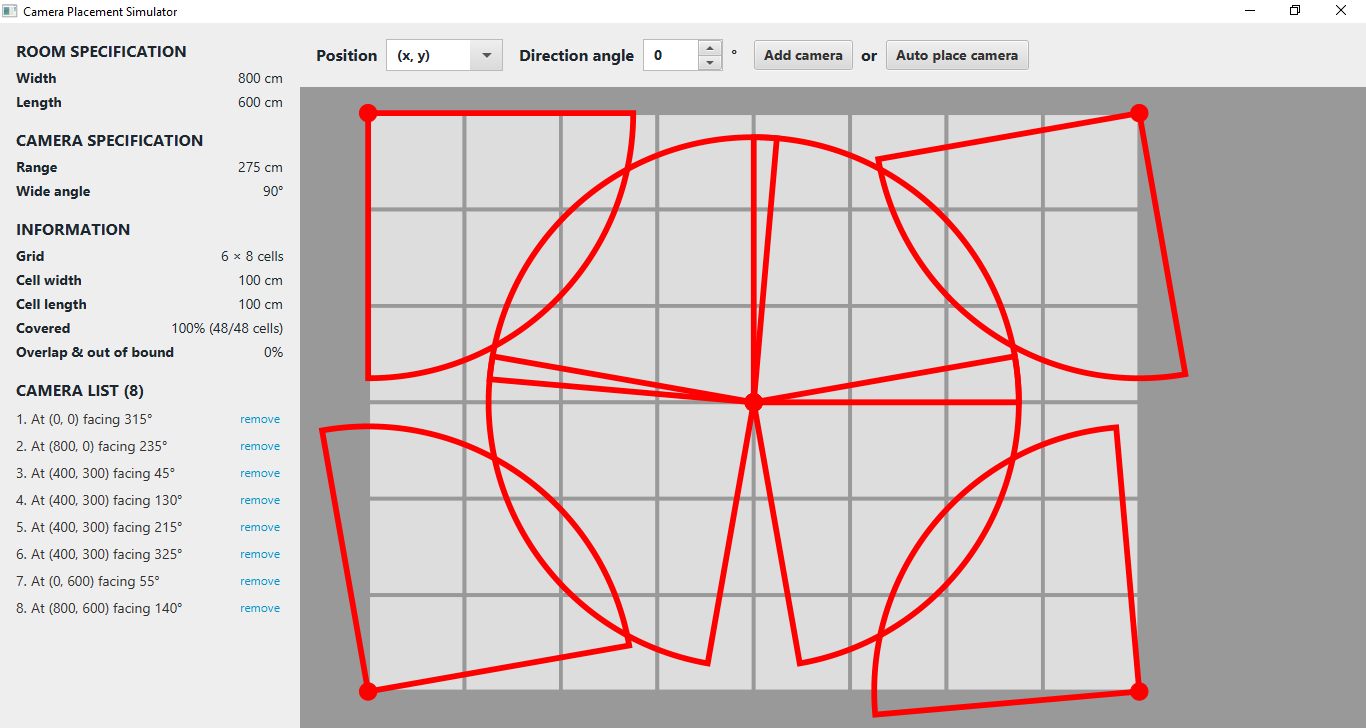
\includegraphics[scale=0.45]{exp_1_1_a}
	\caption[Hasil eksperimen ukuran cell, pertama]{Hasil eksperimen ukuran cell, pertama}
	\label{fig:exp_1_1_a}
\end{figure}

\begin{figure}[H]
	\centering  
	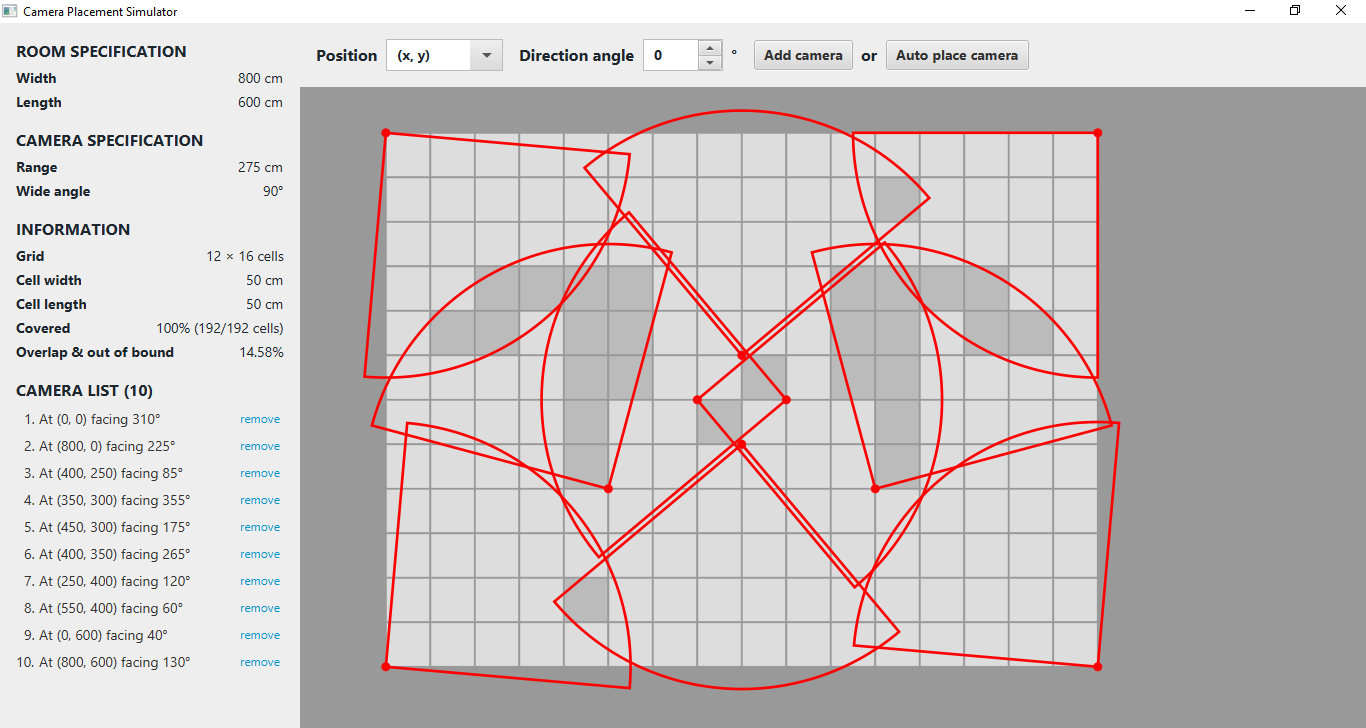
\includegraphics[scale=0.45]{exp_1_1_b}
	\caption[Hasil eksperimen ukuran cell, kedua]{Hasil eksperimen ukuran cell, kedua}
	\label{fig:exp_1_1_b}
\end{figure}

\begin{figure}[H]
	\centering  
	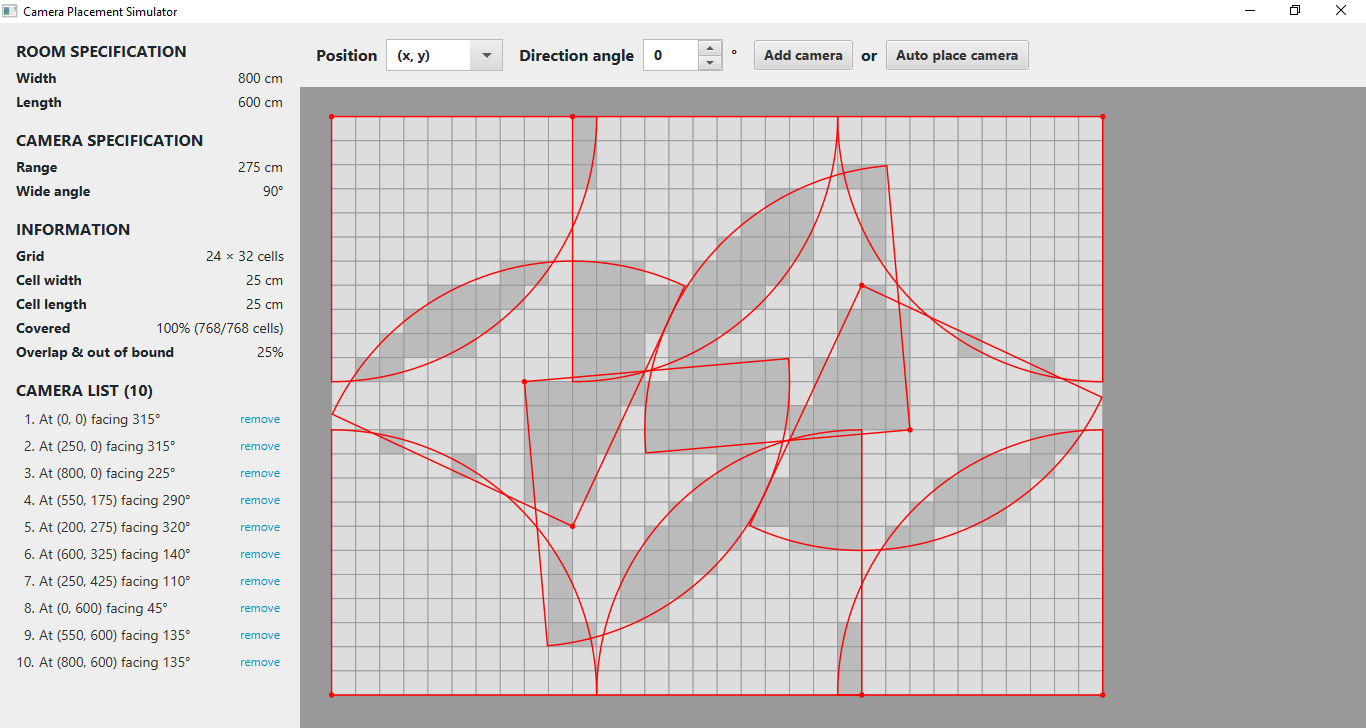
\includegraphics[scale=0.45]{exp_1_1_c}
	\caption[Hasil eksperimen ukuran cell, ketiga]{Hasil eksperimen ukuran cell, ketiga}
	\label{fig:exp_1_1_c}
\end{figure}

\begin{figure}[H]
	\centering  
	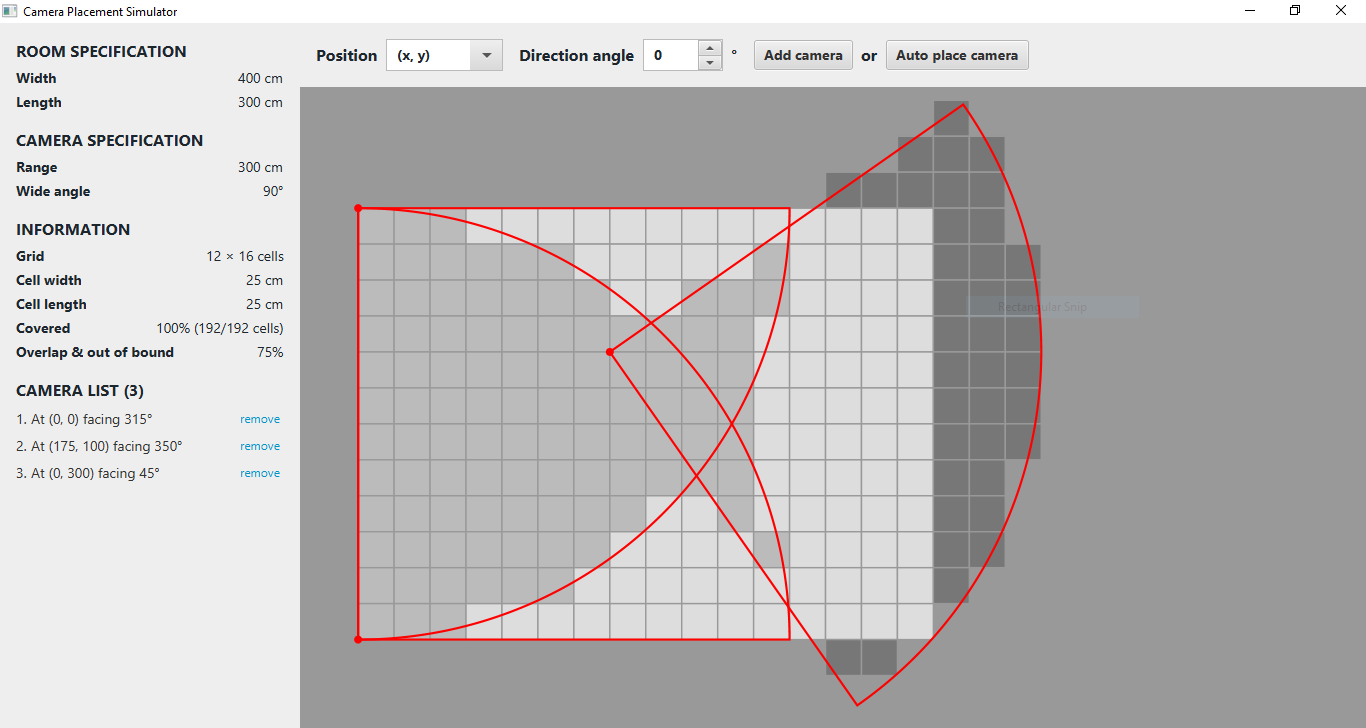
\includegraphics[scale=0.45]{exp_1_2_a}
	\caption[Hasil eksperimen rasio, pertama]{Hasil eksperimen rasio, pertama}
	\label{fig:exp_1_2_a}
\end{figure}

\begin{figure}[H]
	\centering  
	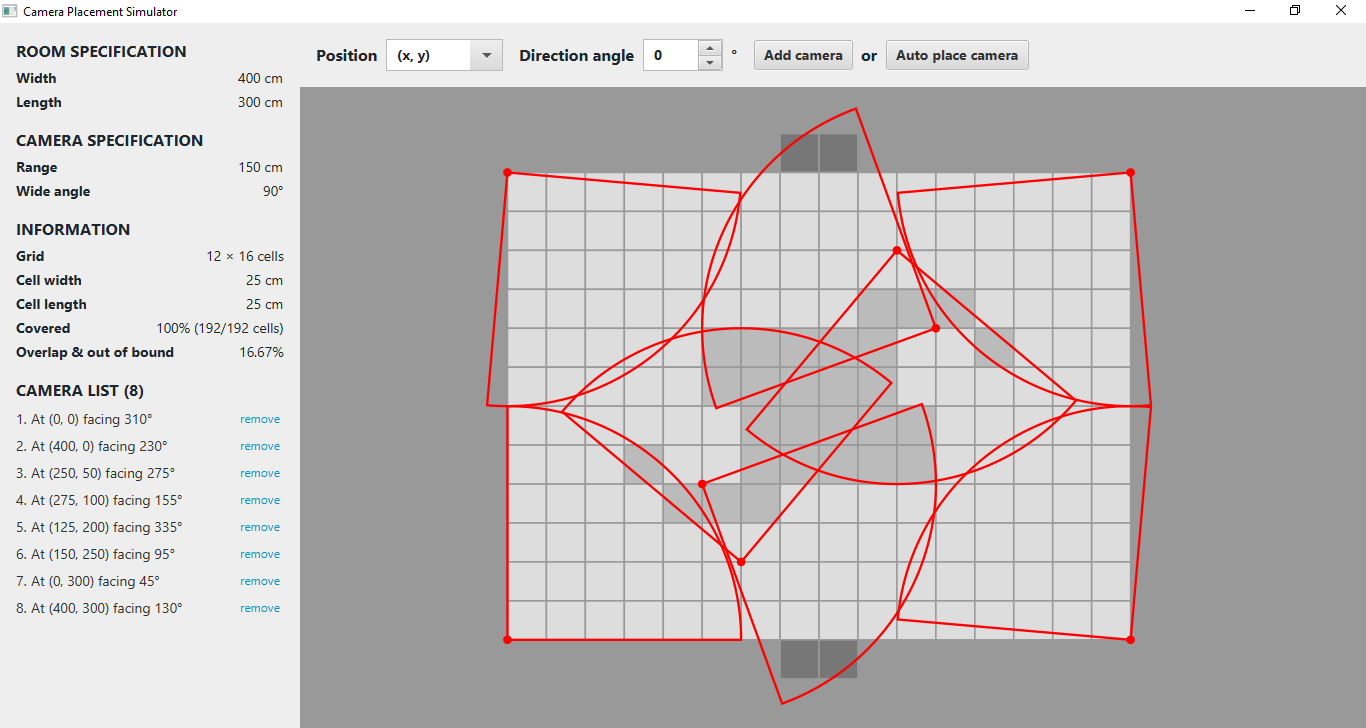
\includegraphics[scale=0.45]{exp_1_2_b}
	\caption[Hasil eksperimen rasio, kedua]{Hasil eksperimen rasio, kedua}
	\label{fig:exp_1_2_b}
\end{figure}

\begin{figure}[H]
	\centering  
	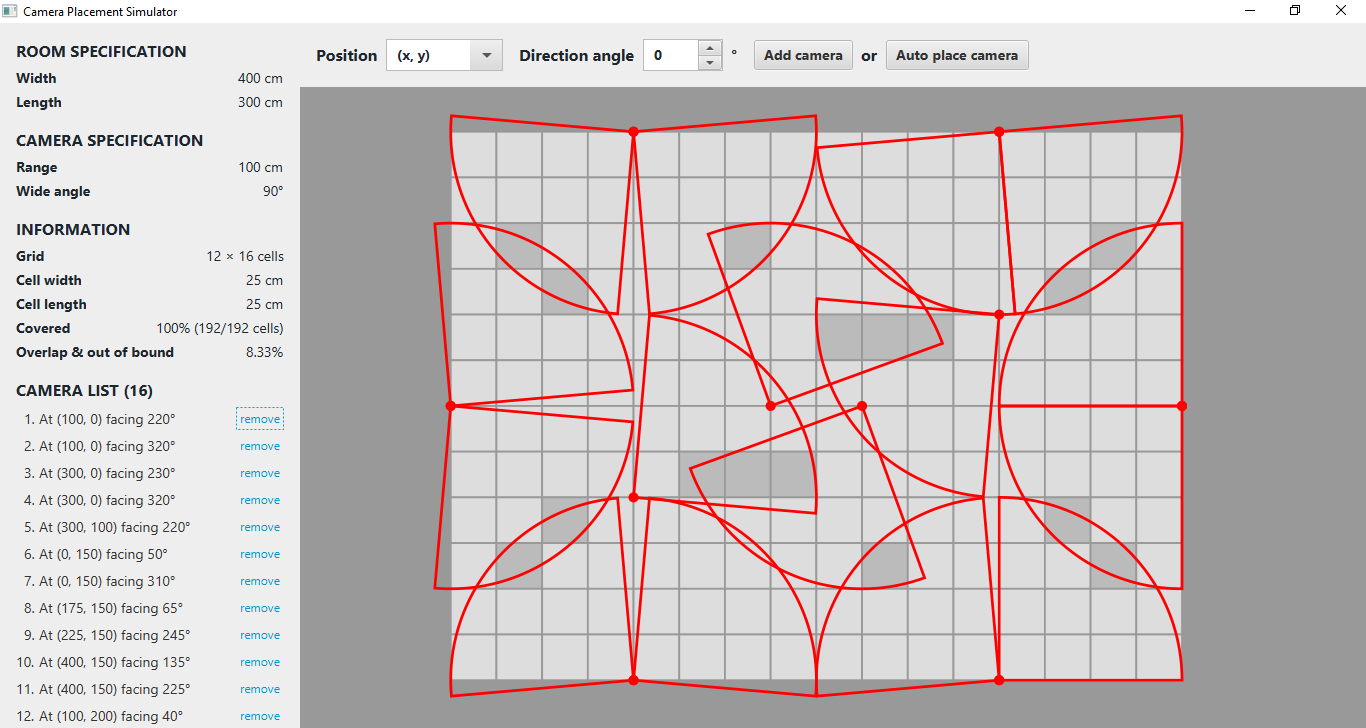
\includegraphics[scale=0.45]{exp_1_2_c}
	\caption[Hasil eksperimen rasio, ketiga]{Hasil eksperimen rasio, ketiga}
	\label{fig:exp_1_2_c}
\end{figure}

\begin{figure}[H]
	\centering  
	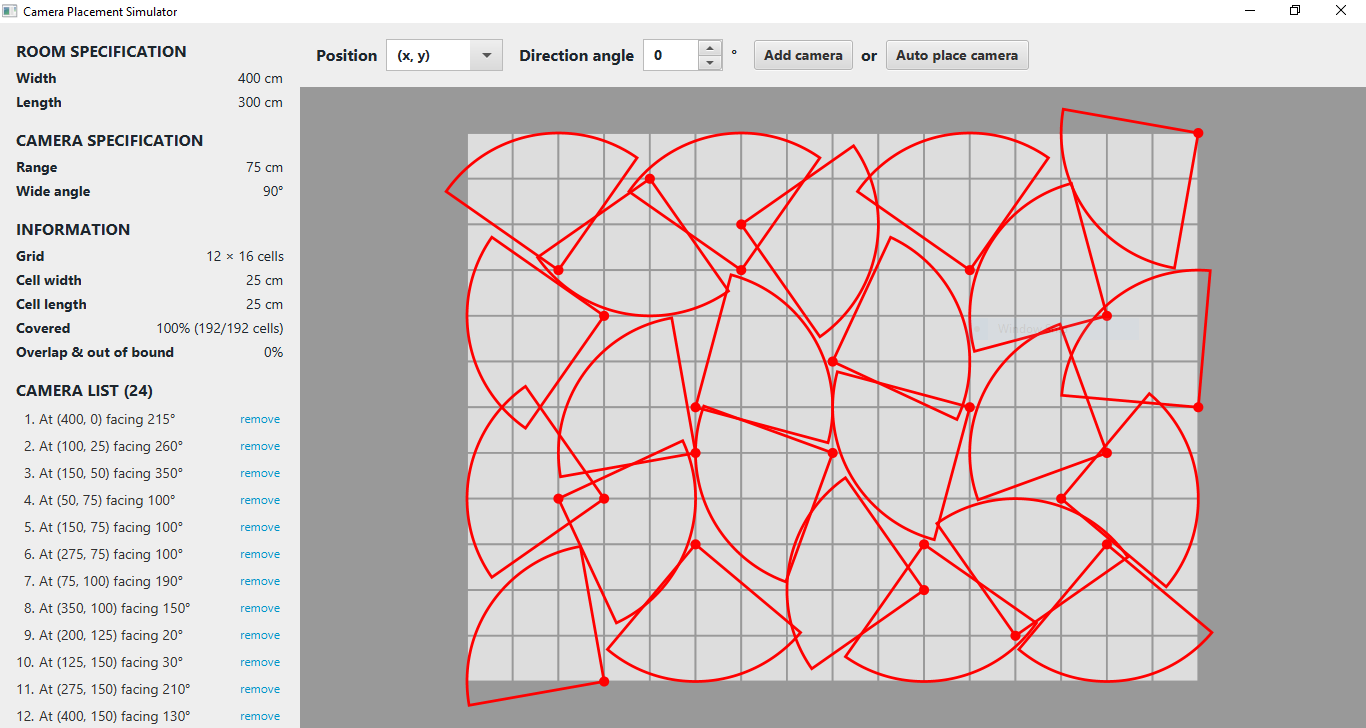
\includegraphics[scale=0.45]{exp_1_2_d}
	\caption[Hasil eksperimen rasio, keempat]{Hasil eksperimen rasio, keempat}
	\label{fig:exp_1_2_d}
\end{figure}

\begin{figure}[H]
	\centering  
	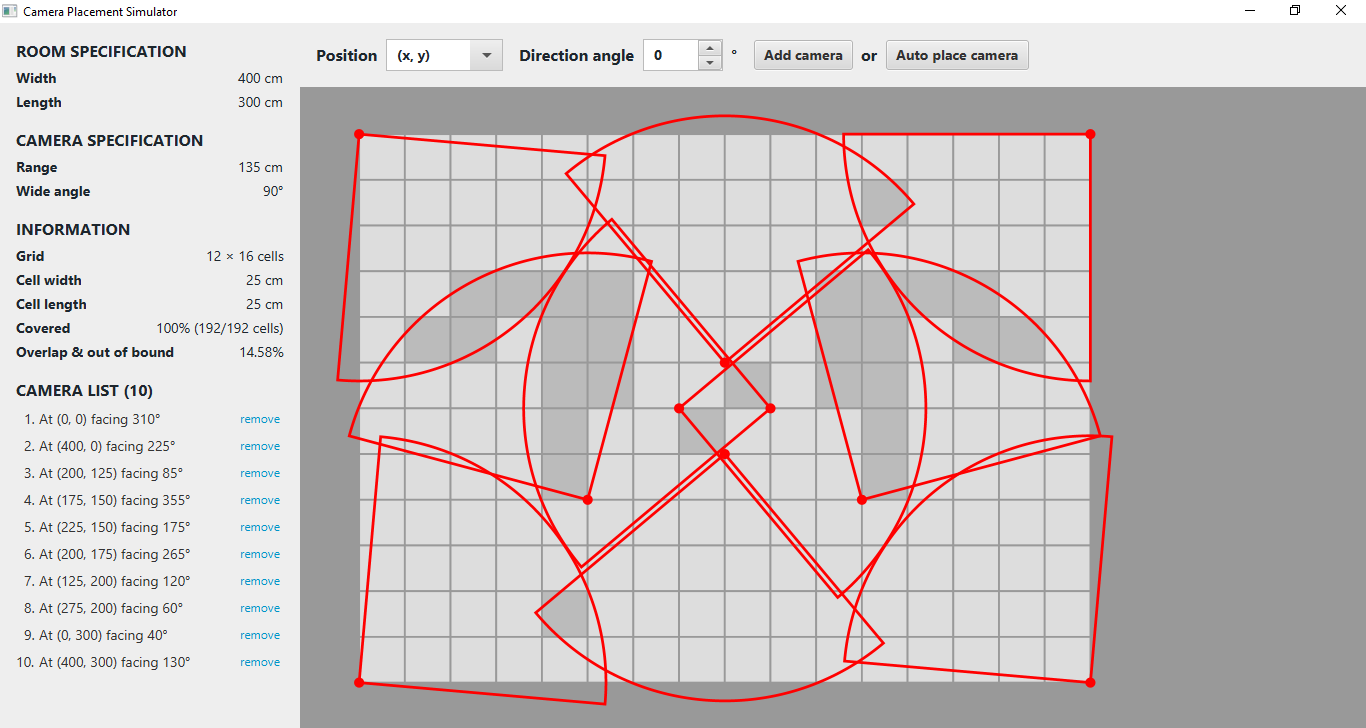
\includegraphics[scale=0.45]{exp_1_3_a}
	\caption[Hasil eksperimen besar sudut pandang, pertama]{Hasil eksperimen besar sudut pandang, pertama}
	\label{fig:exp_1_3_a}
\end{figure}

\begin{figure}[H]
	\centering  
	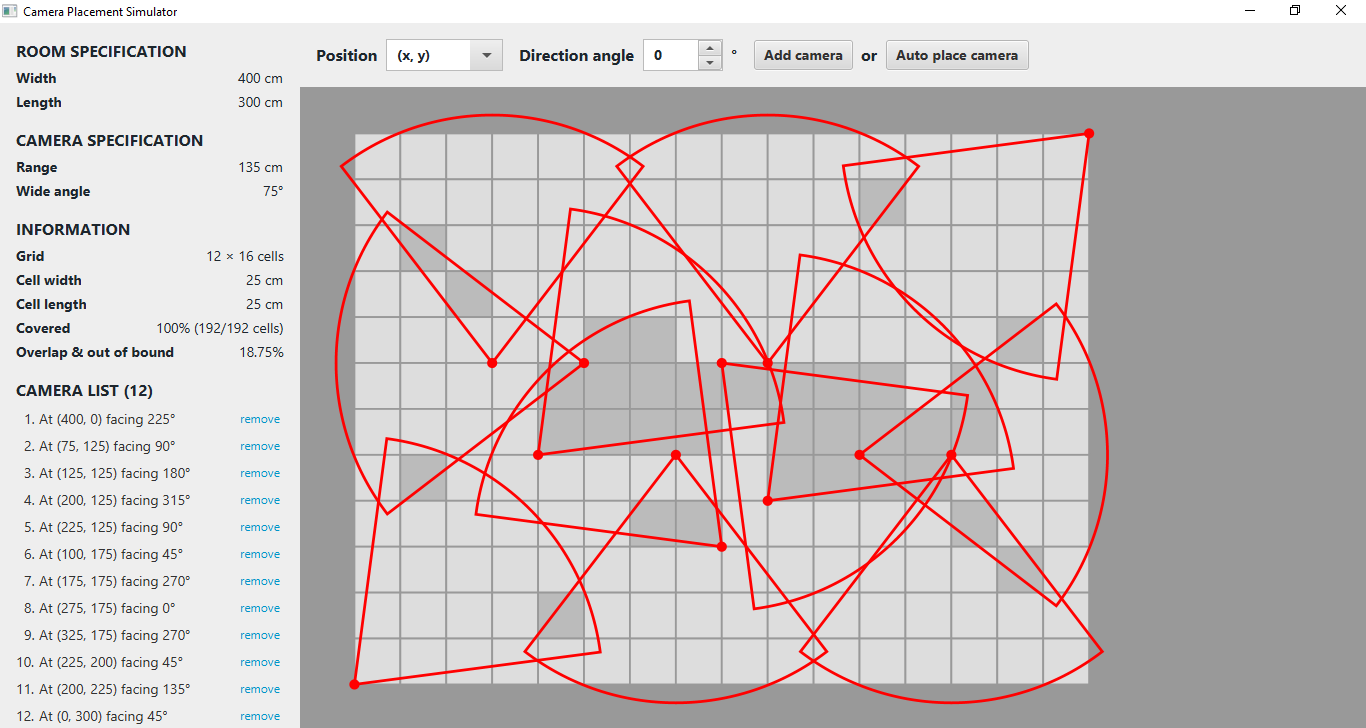
\includegraphics[scale=0.45]{exp_1_3_b}
	\caption[Hasil eksperimen besar sudut pandang, kedua]{Hasil eksperimen besar sudut pandang, kedua}
	\label{fig:exp_1_3_b}
\end{figure}

\begin{figure}[H]
	\centering  
	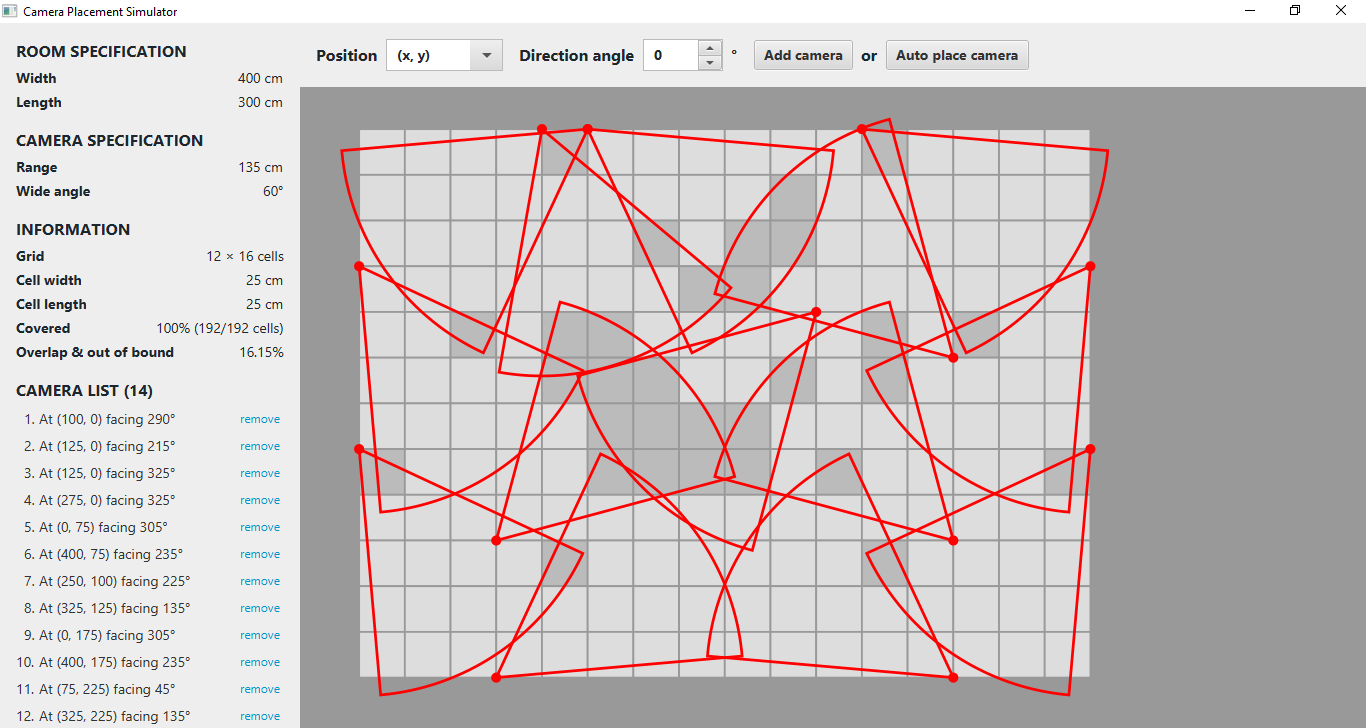
\includegraphics[scale=0.45]{exp_1_3_c}
	\caption[Hasil eksperimen besar sudut pandang, ketiga]{Hasil eksperimen besar sudut pandang, ketiga}
	\label{fig:exp_1_3_c}
\end{figure}

\begin{figure}[H]
	\centering  
	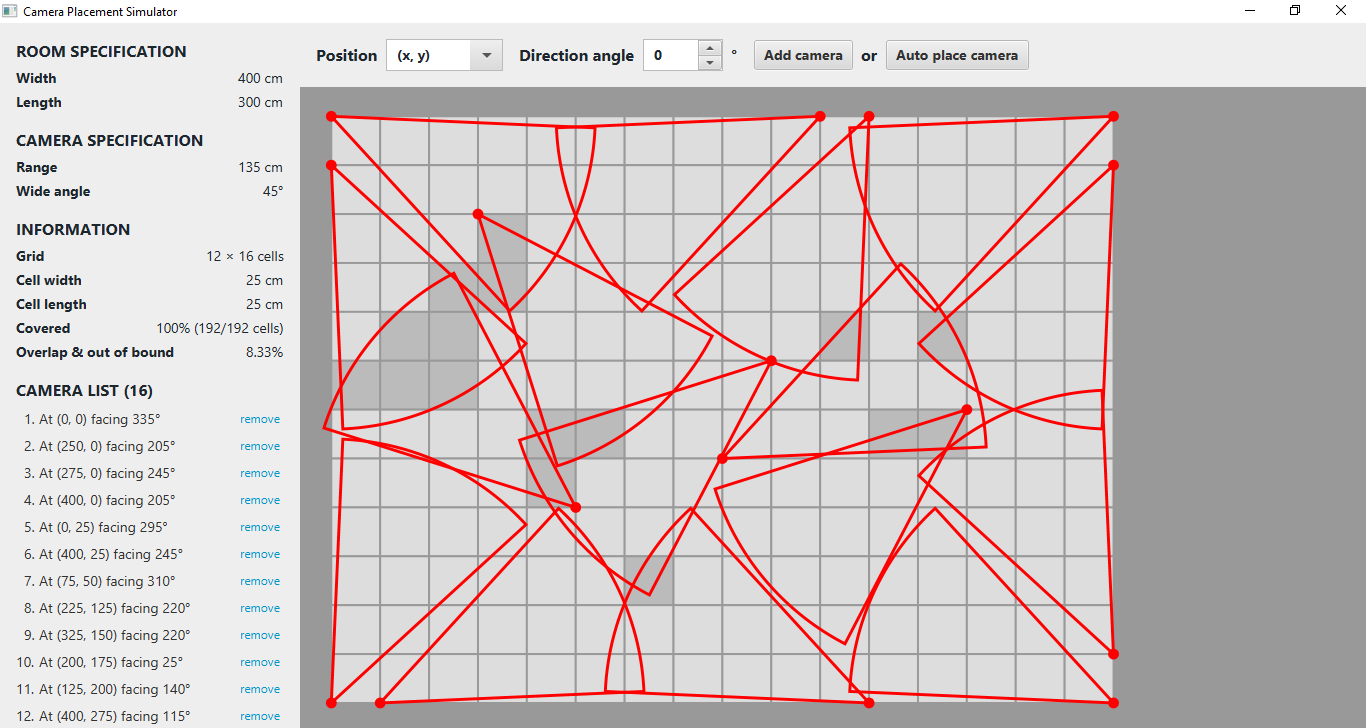
\includegraphics[scale=0.45]{exp_1_3_d}
	\caption[Hasil eksperimen besar sudut pandang, keempat]{Hasil eksperimen besar sudut pandang, keempat}
	\label{fig:exp_1_3_d}
\end{figure}